\subsubsection{Validació del formulari de cerca}

\paragraph{}
A diferència de la funcionalitat de cerca general, aquesta funcionalitat, sí que realitza una validació més exhaustiva dels valors introduïts per l'usuari a través del formulari, ja que una configuració incorrecta d'aquests, resultaria l’obtenció de zero resultats.

Han estat implementades dues menes de validacions diferents. La coneguda com a validació en línia i la validació del formulari quan es prem el botó de cerca.

La validació en línia s'activa quan l'usuari surt d'un camp del formulari i s'aprofita aquest moment, per mostrar el marc del camp, en vermell, si aquest conté algun error, o en verd, si el valor introduït és correcte. L'objectiu d'aquesta validació és facilitar a l'usuari la comprensió dels errors i corregir-los al més aviat possible; reduint així, la frustració en el moment de realitzar la cerca.

Per activar la validació en línia, s'utilitza la funció jQuery \emph{onFocusOut()} en conjunció a les classes de Bootstrap \emph{has-success} o \emph{has-error}, que en ser afegides al camp d'un formulari, en pinten la bora de color verd o vermell de forma respectiva.

\begin{lstlisting}[style=rawOwn,caption={Activació de la validació en línia}]
$(`.form-vali').focusout(function() {
    if(inlineValidation($(this).attr(`id'))) {
        $(this).parent().removeClass(`has-success');
        $(this).parent().addClass(`has-error');
    }
    else {
        $(this).parent().removeClass(`has-error');
        $(this).parent().addClass(`has-success');
}
});
\end{lstlisting}

Com es pot observar en el bloc de codi anterior, per tal de comprovar si un camp és vàlid o no, es crida la funció \emph{inlineValidation(param)}, amb l’identificador del camp a comprovar. Aquesta funció es reutilitza tant per la validació en línia, com per la validació en el moment de cerca.

Les regles de validació per cada un dels camps del formulari s'especifiquen a continuació:

\begin{itemize}
    \item \textbf{Cognom:} Si el paràmetre té longitud zero, es mostra un error.
    \item \textbf{Països:} Si no s'ha seleccionat com a mínim un país, es mostra un error.
    \item \textbf{Any de naixement:} Si la longitud és diferent de quatre o no és un número, es mostra un error.
    \item \textbf{Rang:} Si el camp no està buit i la longitud és diferent de quatre o no és un número, es mostra un error.
    \item \textbf{Interval:} Si els paràmetres \emph{any de naixement} i \emph{rang} són diferents, el paràmetre \emph{rang} no és buit i \emph{l’interval} no està especificat o no és un nombre, es mostra un error.
\end{itemize}

La imatge~\ref{fig:surnamesError}, mostra a la vegada, els errors en línia (marc dels camps del formulari en vermell o verd) i la caixa d'errors que informa l'usuari dels errors produïts, de forma més detallada, quan l’usuari prem el botó de cerca amb paràmetres incorrectes.

\begin{figure}[h]
    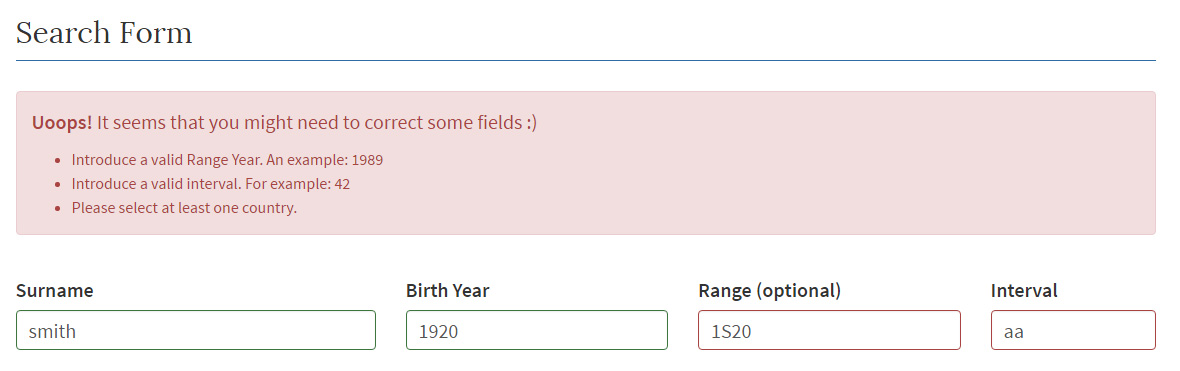
\includegraphics[width=\linewidth]{11/03_surnamesSearch/01_formValidation}
    \centering
    \caption{Exemples d'error en els formularis decerca}\label{fig:surnamesError}
\end{figure}

Si totes les validacions són superades, quan el formulari és enviat cap al SDK, s'escapen els paràmetres llegits de la mateixa forma que s'ha explicat per la funcionalitat de cerca en l’arbre familiar.
